% Paper A: IEEE conference format, at most 7 pages including references (the guide's limit).
% IEEEtran conference, 10pt. The venue is chosen later by the guide; reformat then if needed.
%
% THIS IS A SKELETON. Every \todo{} marks text the AUTHORS write. Bullets inside \todo{} are content points,
% not prose to copy. Section guide: paper_a/02_section_guide.md. Figures and captions: 03_figures_tables.md.
% Every number you may quote, with its source: 05_numbers.md. The tables below already hold the measured
% numbers (from paper_a/figure_data/*.csv); check against 05_numbers.md if you edit them.
%
% Compile on Overleaf (pdfLaTeX): New Project -> Upload Project (zip of paper_a/latex/). BibTeX with refs.bib.

\documentclass[conference,10pt]{IEEEtran}
\IEEEoverridecommandlockouts
\usepackage{cite}
\usepackage{amsmath,amssymb}
\usepackage{graphicx}
\usepackage{booktabs}
\usepackage{multirow}
\usepackage{url}
\usepackage{xcolor}
\usepackage{algorithm}
\usepackage{algpseudocode}
\usepackage{tikz}
\usetikzlibrary{positioning,arrows.meta,fit,backgrounds}
\newcommand{\todo}[1]{\textcolor{red}{[TODO: #1]}}
\DeclareMathOperator*{\clip}{clip}

\begin{document}

\title{\todo{title; ingredients in 01\_story\_and\_claims.md}}

\author{\IEEEauthorblockN{\todo{authors}}
\IEEEauthorblockA{\todo{affiliation}}}

\maketitle

\begin{abstract}
\todo{150--200 words, written LAST. Content points (01\_story\_and\_claims.md, ``Abstract''):
problem (remediation of microservice faults; scripted runbooks are brittle; RL usually trained in simulators);
what we do (online discrete-action RL on a live K3s cluster, guarded by masks and an in-flight lock, 20\,s loop, controller across a wireless edge link);
method in one line (masked discrete SAC with prioritized replay, warm-started from runbook data with behaviour cloning and a conservative critic);
results with numbers (35/40 faults recovered vs 0/40 Kubernetes and 10/40 HPA; median MTTR 79\,s, non-inferior to the runbook; 0/10 false remediations; cold start 15/40 and 10/10 false remediations; replicated on a second seed);
one limitation (one fault/target combination never learned).}
\end{abstract}

\begin{IEEEkeywords}
self-healing systems, reinforcement learning, microservices, Kubernetes, fault remediation, edge computing
\end{IEEEkeywords}

% =====================================================================================================
\section{Introduction}\label{sec:intro}
\todo{$\approx$0.8 page. 02\_section\_guide.md, Section I.
\begin{itemize}
\item Remediation of faults in microservices: MTTR matters; on-call SREs follow runbooks; runbooks are hand-written per fault.
\item RL for cloud control exists (resource management \cite{qiu2020firm,zhang2021sinan}, autoscaling \cite{qiu2023aware}) and for remediation (offline from logs \cite{dai2026saferemediation}; LLM-generated playbooks \cite{zhang2026e2ereme}; guarded planners \cite{habibi2026arbiter,cai2026guardedact}). Gap: a learned \emph{discrete} remediation policy trained \emph{online on the live system}, with hard safety guards, under edge constraints, evaluated against Kubernetes, HPA and a runbook with a pre-registered protocol.
\item Our setting: single-node K3s, Online Boutique, controller on a separate machine over a wireless link, 20\,s real-time control loop.
\item Contributions (numbered list, 4 items): (1) testbed and guarded action interface; (2) agent + warm start; (3) pre-registered evaluation with the results headline; (4) what did not work (cold start, F2-currencyservice) and the open artefacts.
\end{itemize}}

% =====================================================================================================
\section{Related Work}\label{sec:related}
\todo{$\approx$0.5 page. 06\_references.md says what each paper does and how we differ. Three short paragraphs:
\begin{itemize}
\item RL for cloud resource management and autoscaling \cite{qiu2020firm,zhang2021sinan,qiu2023aware}: continuous resource knobs; AWARE bootstraps RL from existing autoscalers, the closest idea to our warm start.
\item Automated remediation \cite{dai2026saferemediation,zhang2026e2ereme,habibi2026arbiter,cai2026guardedact}: offline/CMDP from logs, LLM playbooks, guarded agentic control, sandboxed fixes. We: learned online policy on the live system; guards as hard masks; MTTR and false remediations measured against baselines.
\item Method roots: SAC \cite{haarnoja2018sac}, discrete SAC \cite{christodoulou2019sacd}, PER \cite{schaul2016per}, CQL \cite{kumar2020cql}, action masking \cite{huang2022masking}, learning from demonstrations \cite{hester2018dqfd,nair2020awac}, safe RL \cite{garcia2015saferl}; self-adaptive systems \cite{kephart2003vision}.
\end{itemize}}

% =====================================================================================================
\section{Testbed and Control Loop}\label{sec:testbed}
\todo{$\approx$0.8 page. 04\_methodology\_facts.md, ``Testbed'' and ``Control loop''. Points:
two machines (cluster A, controller B), wireless link, B is the clock authority; Online Boutique \cite{onlineboutique} on K3s \cite{k3s}; 4 managed services; telemetry (Prometheus \cite{prometheus}, Kubernetes API, server-side request logs, Locust \cite{locust}); fault injection (Chaos Mesh \cite{chaosmesh}, API patches, load surge); one-action-at-a-time lock; least-privilege credentials (agent cannot delete pods); faults in Table~\ref{tab:faults}.}

\begin{figure}[t]
\centering
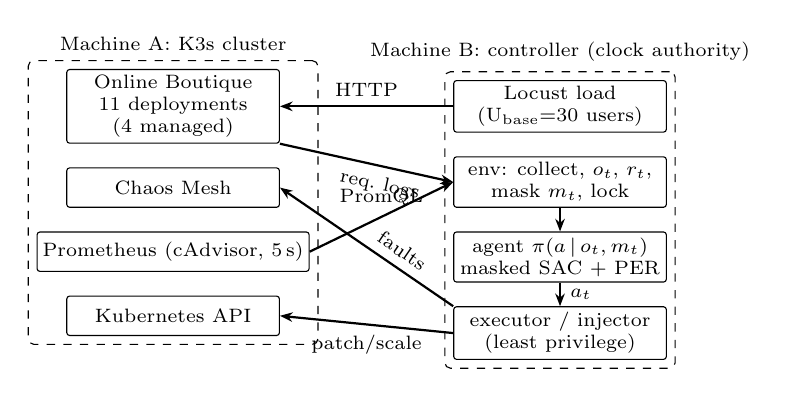
\begin{tikzpicture}[font=\scriptsize, node distance=3mm,
  box/.style={draw, rounded corners=1pt, align=center, inner sep=2pt, minimum height=5mm},
  grp/.style={draw, dashed, rounded corners=2pt, inner sep=3pt},
  arr/.style={-{Stealth[length=1.6mm]}, thick}]
  % Machine A
  \node[box, minimum width=27mm] (ob) {Online Boutique\\11 deployments\\(4 managed)};
  \node[box, below=of ob, minimum width=27mm] (cm) {Chaos Mesh};
  \node[box, below=of cm, minimum width=27mm] (pr) {Prometheus (cAdvisor, 5\,s)};
  \node[box, below=of pr, minimum width=27mm] (api) {Kubernetes API};
  \node[grp, fit=(ob)(cm)(pr)(api), label={above:Machine A: K3s cluster}] (A) {};
  % Machine B
  \node[box, right=22mm of ob, minimum width=27mm] (lo) {Locust load\\(U\textsubscript{base}=30 users)};
  \node[box, below=of lo, minimum width=27mm] (env) {env: collect, $o_t$, $r_t$,\\mask $m_t$, lock};
  \node[box, below=of env, minimum width=27mm] (ag) {agent $\pi(a\,|\,o_t,m_t)$\\masked SAC + PER};
  \node[box, below=of ag, minimum width=27mm] (ex) {executor / injector\\(least privilege)};
  \node[grp, fit=(lo)(env)(ag)(ex), label={above:Machine B: controller (clock authority)}] (B) {};
  % links
  \draw[arr] (lo.west) -- node[above]{HTTP} (ob.east);
  \draw[arr] (pr.east) -- node[above]{PromQL} (env.west);
  \draw[arr] (ob.south east) -- node[pos=0.6, below, sloped]{req.\ logs} (env.west);
  \draw[arr] (env) -- (ag);
  \draw[arr] (ag) -- node[right]{$a_t$} (ex);
  \draw[arr] (ex.west) -- node[below]{patch/scale} (api.east);
  \draw[arr] (ex.north west) -- node[pos=0.35, above, sloped]{faults} (cm.east);
\end{tikzpicture}
\caption{\todo{caption facts in 03\_figures\_tables.md, Fig.~1: two machines over a wireless link; one tick every 20\,s; collect within 3\,s; one action in flight.}}
\label{fig:arch}
\end{figure}

\begin{table}[t]
\centering
\caption{\todo{caption: injected faults, cure condition and the curing action}}
\label{tab:faults}
\setlength{\tabcolsep}{3pt}
\begin{tabular}{@{}llll@{}}
\toprule
Fault & Injection & Cure condition & Curing action \\
\midrule
F1 bad deploy & \texttt{EXTRA\_LATENCY} 0.3/0.6/1\,s on pc & template = golden & RESTORE pc \\
F2 hot pod & CPU stress, 1/2 workers, cart/curr & stressed pod gone & RESTART X \\
F3 scaled to 0 & cart/curr $\rightarrow$ 0 replicas & $\geq$1 available & RESTORE/SCALE X \\
F4 surge & load $\times$2.5/$\times$3.0 & SLA only & SCALE\_UP fe \\
NULL & none & -- & NOOP \\
\bottomrule
\end{tabular}
\end{table}

% =====================================================================================================
\section{Remediation as a Masked MDP}\label{sec:method}
\todo{$\approx$1.3 pages with the equations and Algorithm~\ref{alg:loop}. 04\_methodology\_facts.md, ``MDP'' and ``Agent''. Explain each equation in one or two sentences of your own.}

\paragraph*{Observation and actions}
\todo{36 features (5 global, 7 per managed service, 3 controller); 12 actions (NOOP, 4 RESTART, 3 SCALE\_UP, SCALE\_DOWN frontend, 3 RESTORE). No ground truth in $o_t$ or $m_t$.}
The latency feature, with $L$ the server-side p95 latency and $L_{\mathrm{SLA}}=70$\,ms:
\begin{equation}
o_t^{\mathrm{lat}} = \clip\!\Big(\tfrac{\log_2(1+L_t/L_{\mathrm{SLA}})}{\log_2 21},\,0,\,1\Big).
\end{equation}

\paragraph*{Mask and lock}
\begin{equation}
m_t(a)=\begin{cases}
1 & a=\textsc{noop}\\
0 & \text{lock held}\\
\mathbf{1}[\text{replica bounds and target state allow }a] & \text{otherwise}
\end{cases}
\end{equation}
\todo{lock clears on rollout complete, 100\,s timeout or dispatch error; bounds enforced twice (mask and executor); RESTORE never masked by drift (would leak the fault).}

\paragraph*{Reward and recovery}
With failure ratio $F_t$, $e_{\mathrm{sla}}=0.01$, $e_{\max}=0.20$:
\begin{align}
\ell_t &= \clip\big(\log_2(L_t/L_{\mathrm{SLA}})/3,\,0,\,1\big),\quad
e_t = \clip\Big(\tfrac{F_t-e_{\mathrm{sla}}}{e_{\max}-e_{\mathrm{sla}}},0,1\Big),\\
v_t &= \clip(\ell_t+e_t,0,1),\qquad
\rho_t=\tfrac{1}{4}\textstyle\sum_d \max(0,\mathit{spec}_d-\mathit{base}_d),\\
r_k &= -\big(v_{k+1} + c(a_k) + 0.05\,\rho_{k+1}\big),\quad r_k\in[-1.09,0],
\end{align}
with $c(\textsc{noop})=0$, $c(\textsc{scale})=0.02$, $c(\textsc{restart})=c(\textsc{restore})=0.04$.
A tick is healthy, $H_t$, iff $L_t\le L_{\mathrm{SLA}}$ and $F_t\le e_{\mathrm{sla}}$. An episode recovers at the first tick $t$ after injection with $H_t\wedge H_{t+1}\wedge H_{t+2}$ and the fault's cure condition (Table~\ref{tab:faults}):
\begin{equation}
\mathrm{MTTR}=\mathrm{wall}(T_t)-t_{\mathrm{inject}},\quad \text{censored at } 360\,\mathrm{s}.
\end{equation}

\paragraph*{Masked discrete SAC}
\begin{align}
\pi_\phi(a\,|\,s) &= \mathrm{softmax}\big(z_\phi(s)\odot m + (-10^9)(1-m)\big)_a,\\
V(s') &= \textstyle\sum_{a:\,m'(a)=1}\pi(a|s')\big[\min_j \bar Q_j(s',a) - \alpha\log\pi(a|s')\big],\\
y &= \textstyle\sum_{i=0}^{n-1}\gamma^i r_{t+i} + \gamma^n (1-d_{t+n})\,V(s_{t+n}),\\
\mathcal{L}_\pi &= \mathbb{E}_s\textstyle\sum_{a:\,m(a)=1}\pi(a|s)\big[\alpha\log\pi(a|s)-\min_j Q_j(s,a)\big],
\end{align}
with masked log-probabilities set to zero before any $\pi\log\pi$ product; $\gamma=0.93$, $n=3$, $d$ = terminated (bootstrap on truncation).

\paragraph*{Conservative critic and prioritized replay}
\begin{align}
\mathcal{L}_Q &= \mathbb{E}_i\big[w_i\,(Q_j(s_i,a_i)-y_i)^2\big]
 + \lambda\,\mathbb{E}_s\Big[\log\!\!\sum_{a:\,m(a)=1}\!\! e^{Q_j(s,a)} - Q_j(s,a_{\mathcal D})\Big],\\
P(i) &= \frac{p_i^{\beta_p}}{\sum_k p_k^{\beta_p}},\quad
p_i=\min\big(\tfrac{|\delta_{1,i}|+|\delta_{2,i}|}{2},1\big)+\epsilon,\quad
w_i=\frac{(N P(i))^{-\beta}}{\max_k w_k},
\end{align}
$\lambda=1$, $\beta_p=0.5$, $\beta$: $0.4\rightarrow1$ over 15\,000 gradient steps, $\alpha$ fixed at 0.1 online. \todo{why CQL + fixed $\alpha$ (Amendments 5--6: extrapolation error made the agent act in healthy states); why warm start: behaviour cloning of the actor on 120 runbook episodes with $\varepsilon=0.25$ exploration, 2000 offline steps. Note: our PER priority exponent is written $\beta_p$ here to avoid a clash with SAC's $\alpha$; the contract calls it \texttt{per.alpha}.}

\begin{table}[t]
\centering
\caption{\todo{caption: agent hyper-parameters (locked in the contract before training)}}
\label{tab:hparams}
\setlength{\tabcolsep}{3pt}
\begin{tabular}{@{}ll@{}}
\toprule
Networks & actor, twin critics: MLP $36\rightarrow256\rightarrow256\rightarrow12$, ReLU \\
$\gamma$, $n$-step, $\tau$ & 0.93, 3, 0.005 \\
Learning rates & $3\times10^{-4}$ (actor, critics) \\
Batch, buffer & 128, 50\,000 \\
Updates per tick & 4 (budget 1\,s) \\
Temperature $\alpha$ & fixed 0.1 online \\
CQL weight $\lambda$ & 1.0 (offline and online) \\
PER & $\beta_p=0.5$, $\beta$ $0.4\rightarrow1$ (15\,000 steps), $\epsilon=10^{-3}$, cap 1 \\
Warm start & 120 runbook episodes ($\varepsilon=0.25$), 2000 offline steps (BC + CQL) \\
Training & 200 online episodes per seed; final checkpoint evaluated \\
\bottomrule
\end{tabular}
\end{table}

\begin{algorithm}[t]
\caption{One tick of the guarded control loop (20\,s)}\label{alg:loop}
\small
\begin{algorithmic}[1]
\State $a \gets \arg\max_a$ / sample $\pi(\cdot\,|\,o_k, m_k)$ \Comment{masked}
\If{$m_k(a)=0$} \State $a\gets\textsc{noop}$ \EndIf
\If{$a\neq\textsc{noop}$} \State acquire lock; dispatch $a$ asynchronously \EndIf
\State sleep until $T_{k+1}=T_0+(k+1)\cdot 20$\,s
\State collect Locust, PromQL, Kubernetes, server logs concurrently (deadline 3\,s)
\State release lock if target rollout complete, timeout, or dispatch error
\State $o_{k+1}\gets$ normalize and impute; $r_k\gets$ reward; $m_{k+1}\gets$ mask
\If{$o_{k+1}$ not stale} \State store $(o_k,a_{\mathrm{exec}},r_k,o_{k+1},m_{k+1})$ with max priority \EndIf
\State 4 gradient steps (budget 1\,s)
\end{algorithmic}
\end{algorithm}

% =====================================================================================================
\section{Experimental Design}\label{sec:design}
\todo{$\approx$0.7 page. 04\_methodology\_facts.md, ``Baselines'' and ``Evaluation protocol''. Points:
baselines (Kubernetes default, Kubernetes + HPA \cite{k8shpa}, scripted runbook with 7 ordered rules on the same observation); pre-registration before training, with 8 dated amendments (list the substantive ones in one sentence each); schedule eval\_v1 (50 entries: 10 per fault type + 10 NULL, seed 2026), interleaved policies; edge subset (20 entries, netem \cite{hemminger2005netem} +150\,ms and 1\,\% loss on control-plane traffic only); seed-1 replication with a same-block runbook anchor; statistics: Mann--Whitney U \cite{mann1947test}, Holm \cite{holm1979simple}, Cliff's $\delta$ \cite{cliff1993dominance}, bootstrap CIs \cite{efron1993bootstrap}, Kaplan--Meier and log-rank \cite{kaplan1958nonparametric}; non-inferiority margin 20\,s (one tick); hypotheses in Table~\ref{tab:hyp}.}

% =====================================================================================================
\section{Results}\label{sec:results}
\todo{$\approx$2 pages including figures/tables. 03\_figures\_tables.md says what each one shows and what to say. Order: Table~\ref{tab:main} + Fig.~\ref{fig:km} (H1, H2) $\rightarrow$ Table~\ref{tab:actions} (what the agent learned) $\rightarrow$ Fig.~\ref{fig:train} (H3) $\rightarrow$ safety (H4) $\rightarrow$ Fig.~\ref{fig:edge} (H5) $\rightarrow$ seed 1 (Table~\ref{tab:seed1}) $\rightarrow$ Table~\ref{tab:hyp} summary.}

\begin{table}[t]
\centering
\caption{\todo{caption: main evaluation, 10 episodes per fault and policy; MTTR median with non-recovered episodes censored at 360\,s; in brackets the median over recovered episodes only}}
\label{tab:main}
\setlength{\tabcolsep}{2.5pt}
\begin{tabular}{@{}lccccc@{}}
\toprule
 & Kubernetes & K8s + HPA & Runbook & PER-SAC & PER-SAC \\
 & & & & (warm) & (cold) \\
\midrule
\multicolumn{6}{@{}l}{\emph{Recovered (of 10)}}\\
F1 & 0 & 0 & 10 & 10 & 0 \\
F2 & 0 & 0 & 8 & 5 & 0 \\
F3 & 0 & 0 & 10 & 10 & 5 \\
F4 & 0 & 10 & 10 & 10 & 10 \\
F1--F4 & 0/40 & 10/40 & 38/40 & 35/40 & 15/40 \\
\midrule
\multicolumn{6}{@{}l}{\emph{Median MTTR, s (censored at 360)}}\\
F1 & 360 & 360 & 80 & 59 & 360 \\
F2 & 360 & 360 & 89 & 240 & 360 \\
F3 & 360 & 360 & 50 & 60 & 230 \\
F4 & 360 & 59 & 80 & 60 & 60 \\
F1--F4 & 360 & 360 & 80 (80) & 79 (60) & 360 (60) \\
\midrule
SLA penalty, mean & 11.44 & 10.26 & 2.18 & 2.25 & 8.39 \\
Actions / fault ep. & 0 & 0 & 1.23 & 1.13 & 17.7 \\
NULL eps.\ with action & 0/10 & 0/10 & 0/10 & 0/10 & 10/10 \\
\bottomrule
\end{tabular}
\end{table}

\begin{figure}[t]
\centering
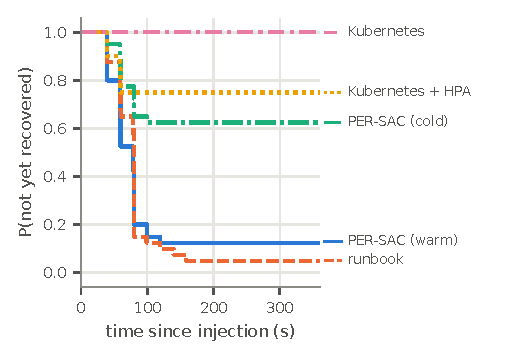
\includegraphics[width=\columnwidth]{figures/a1_km.pdf}
\caption{\todo{caption facts in 03\_figures\_tables.md, Fig.~2 (pooled F1--F4 Kaplan--Meier; log-rank vs PER-SAC: Kubernetes $p<10^{-16}$, HPA $p=2.3\times10^{-7}$, cold $p=3.3\times10^{-6}$, runbook $p=0.95$)}}
\label{fig:km}
\end{figure}

\begin{figure*}[t]
\centering
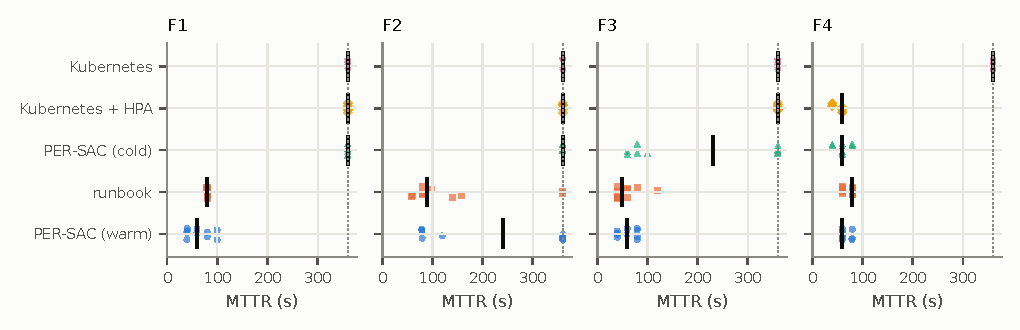
\includegraphics[width=\textwidth]{figures/a2_mttr_by_fault.pdf}
\caption{\todo{caption facts in 03\_figures\_tables.md, Fig.~3 (dots = episodes, bar = median, dotted line = 360\,s censoring)}}
\label{fig:byfault}
\end{figure*}

\begin{table}[t]
\centering
\caption{\todo{caption: executed actions per fault in the main evaluation (episodes); ``none'' = no action}}
\label{tab:actions}
\setlength{\tabcolsep}{3pt}
\begin{tabular}{@{}lll@{}}
\toprule
Fault (target) & PER-SAC (warm) & Runbook \\
\midrule
F1 (pc) & RESTORE pc 8, $\times$2: 2 & RESTORE pc 10 \\
F2 (cart) & RESTART cart 5 & RESTART cart 5 \\
F2 (curr) & none 5 & RESTART curr 3, none 2 \\
F3 (cart) & RESTORE cart 5 & RESTORE cart 4, +RESTART 1 \\
F3 (curr) & RESTORE curr 5 & RESTORE curr 5 \\
F4 (fe) & SCALE\_UP fe $\times$2: 8, $\times$1: 2 & SCALE\_UP fe $\times$2: 10 \\
NULL & none 10 & none 10 \\
\bottomrule
\end{tabular}
\end{table}

\begin{figure}[t]
\centering
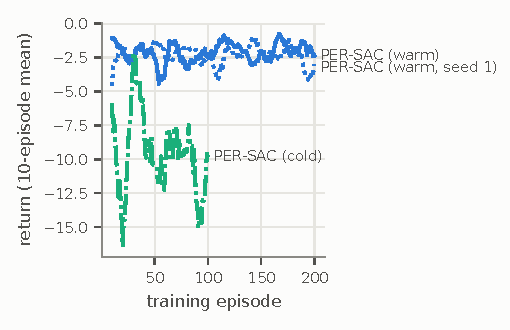
\includegraphics[width=\columnwidth]{figures/a3_training.pdf}
\caption{\todo{caption facts in 03\_figures\_tables.md, Fig.~4 (10-episode rolling mean return; cold start ran 100 episodes, Amendment 7)}}
\label{fig:train}
\end{figure}

\begin{figure}[t]
\centering
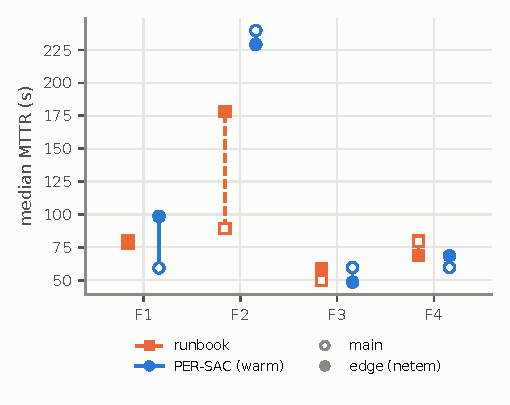
\includegraphics[width=\columnwidth]{figures/a4_edge.pdf}
\caption{\todo{caption facts in 03\_figures\_tables.md, Fig.~5 (4 episodes per fault and condition; hollow = main, filled = netem)}}
\label{fig:edge}
\end{figure}

\begin{table}[t]
\centering
\caption{\todo{caption: seed-1 replication block (50 entries) with the runbook as same-block anchor}}
\label{tab:seed1}
\setlength{\tabcolsep}{3pt}
\begin{tabular}{@{}lcccc@{}}
\toprule
 & \multicolumn{2}{c}{Main block} & \multicolumn{2}{c}{Seed-1 block} \\
 & Runbook & PER-SAC s0 & Runbook & PER-SAC s1 \\
\midrule
Recovered F1--F4 & 38/40 & 35/40 & 37/40 & 35/40 \\
Median MTTR (s) & 80 & 79 & 80 & 80 \\
\quad over recovered & 80 & 60 & 80 & 79 \\
NULL with action & 0/10 & 0/10 & 0/10 & 0/10 \\
H2 CI of median diff.\ (s) & \multicolumn{2}{c}{$[-20.0,\ 0.9]$} & \multicolumn{2}{c}{$[-0.7,\ 19.9]$} \\
\bottomrule
\end{tabular}
\end{table}

\begin{table}[t]
\centering
\caption{\todo{caption: pre-registered hypotheses and outcomes}}
\label{tab:hyp}
\setlength{\tabcolsep}{2.5pt}
\begin{tabular}{@{}p{0.07\columnwidth}p{0.47\columnwidth}p{0.4\columnwidth}@{}}
\toprule
 & Hypothesis & Outcome \\
\midrule
H1 & lower MTTR than Kubernetes and HPA, F1--F4 & supported F1--F3 ($p_{\mathrm{Holm}}\le0.03$); \textbf{not on F4 vs HPA} (HPA faster, $\delta=-0.58$, $p=0.031$) \\
H2 & MTTR non-inferior to runbook (20\,s); lower SLA penalty & non-inferior (CI $[-20.0, 0.9]$\,s); SLA penalty tie ($p=0.66$) \\
H3 & warm start: higher return (ep.\ 1--100), lower MTTR & supported ($p=6.5\times10^{-9}$; MTTR $p=4.4\times10^{-5}$) \\
H4 & no safety violations; 0/10 NULL actions; FRR $\le$10\,\% & supported (0 violations; 0/10; 0/30 training) \\
H5 & edge gap within margin & \textbf{not established} (CI $[-20.1, 20.2]$\,s, margin 20; $n=16$) \\
\bottomrule
\end{tabular}
\end{table}

% =====================================================================================================
\section{Discussion and Limitations}\label{sec:discussion}
\todo{$\approx$0.7 page. 01\_story\_and\_claims.md, ``What the results mean'' and ``Limitations''. Points:
\begin{itemize}
\item The agent learned the runbook's mapping (Table~\ref{tab:actions}) and was faster on F1 and F4 (one tick), never on F2-currencyservice: no exploration with fixed $\alpha$ + CQL (Amendment 6); same blind spot in seed 1.
\item HPA beats both on F4 (reacts without the 2-tick unhealthy debounce, 4/10 at 40\,s) and does nothing else.
\item Warm start is necessary: the cold agent learned a no-op habit (repeated RESTORE cartservice, which is a no-API-call action), 10/10 false remediations.
\item Edge: medians unchanged, decision latency 0.33$\rightarrow$1.44\,s median, but $n=16$ is too small for the 20\,s margin.
\item Limitations: single node, one application, 2 training seeds, shared warm-start data, 20\,s MTTR resolution, near-SLA F2 severity, measurement gaps after scale-from-zero (6 invalid episodes), cold start only 100 episodes, uniform-replay ablation not run so no claim about PER itself.
\end{itemize}}

% =====================================================================================================
\section{Conclusion}\label{sec:conclusion}
\todo{$\approx$0.2 page: what we showed, with two numbers; what is next (exploration for unseen fault/target pairs, multi-node, more seeds).}

\section*{Acknowledgment}
\todo{AI-assistance disclosure in the venue's required wording (07\_format\_and\_submission.md).}

\nocite{*} % TEMPORARY: lists every reference while drafting. DELETE once the text cites with \cite{}.
\bibliographystyle{IEEEtran}
\bibliography{refs}

\end{document}
